\section{eLSA}
    
    In this section we present accuracy achieved by our approach.
    
    Note that because we test on multiple datasets and we test multiple parameters, we witness a small combinatorial explosion.

    \subsection{Parameters}
    
    As mentioned in section \ref{sec:hyperparams}, there is a number of potential hyperparameters. 
    However we consider only the $w'$-learning rate $\beta$ and the number of dimensions.
    Instead of performing an exhaustive hyperparameter search, we test multiple combinations of weighting schemes described in sections \ref{sec:supervised:weights} and \ref{sec:term:weights} on multiple datasets. 

    \begin{table}[H]
\begin{center}
\begin{tabular}{l|l}
\toprule
\midrule
weighting schemes & \texttt{tfidf}, \texttt{tfchi2}, \texttt{tfig}, \texttt{tfgr}, \texttt{tfor}, \texttt{tfrf}, \texttt{None} \\
embedding size & $200$, $300$, $400$ \\
$w'$-learning rates $\beta$ & $0.1$, $0.01$, $0.001$\\
\bottomrule
\end{tabular}
\caption[Table of experiment parameters]{Table of experiment parameters}
\label{tab:exp:params}
\end{center}
\end{table}
    
    We perform experiments with all combinations of parameters from table \ref{tab:exp:params} on all of the $10$ datasets described in section \ref{sec:data:overview}.
    Together we need to perform and evaluate around $630$ experiments.
    
    We compare our results against LSA baseline (LSA with given weights, but without training) and report relative improvements.
    Results for this baseline are in section \ref{sec:lsa:baseline}.
    
    \subsection{Batch gradient descent}
    We evaluate the performance of batch gradient descent optimization routine.
    We perform experiments for different weighting schemes, different sizes of embeddings and different learning rates on all datasets.

    Our results are in the table \ref{tab:batch:results} and table \ref{tab:batch:results:trec}.
    We present only results for $\beta=0.1$, as this learning rate showed to be the best. 
    Experiments for other learning rates can be found in appendix \ref{appendix:detailed}.
    
    
\begin{table}[H]
\begin{center}

\begin{tabular}{ll|rrrr}
\toprule
   &   &   CR &  MPQA &   MR &  SUBJ \\
scheme & lsa &        &        &        &        \\
\midrule
None & 200 & \textbf{0.01} & \textbf{0.02} & \textbf{0.06} & \textbf{0.02} \\
   & 300 & \textbf{0.02} & \textbf{0.02} & \textbf{0.05} &     -0.0 \\
   & 400 & \textbf{0.03} & \textbf{0.01} & \textbf{0.04} & \textbf{0.01} \\
tfchi2 & 200 & \textbf{0.01} &      0.0 & \textbf{0.01} & \textbf{0.01} \\
   & 300 &      0.0 &     -0.0 & \textbf{0.02} & \textbf{0.01} \\
   & 400 & \textbf{0.01} &      0.0 & \textbf{0.03} & \textbf{0.02} \\
tfgr & 200 & \textbf{0.01} &     -0.0 & \textbf{0.01} & \textbf{0.02} \\
   & 300 & \textbf{0.01} &     -0.0 & \textbf{0.01} & \textbf{0.01} \\
   & 400 & \textbf{0.03} & \textbf{0.01} & \textbf{0.01} & \textbf{0.02} \\
tfidf & 200 & \textbf{0.04} & \textbf{0.06} & \textbf{0.07} & \textbf{0.01} \\
   & 300 &     -0.0 & \textbf{0.05} & \textbf{0.05} &      0.0 \\
   & 400 &     -0.01 & \textbf{0.03} & \textbf{0.02} & \textbf{0.01} \\
tfig & 200 &      0.0 & \textbf{0.01} & \textbf{0.01} &     -0.0 \\
   & 300 &      0.0 & \textbf{0.01} & \textbf{0.01} & \textbf{0.01} \\
   & 400 & \textbf{0.03} &      0.0 & \textbf{0.02} & \textbf{0.01} \\
tfor & 200 & \textbf{0.01} &      0.0 &      0.0 & \textbf{0.01} \\
   & 300 &      0.0 &      0.0 &     -0.0 &      0.0 \\
   & 400 &     -0.0 & \textbf{0.02} &     -0.03 & \textbf{0.01} \\
tfrf & 200 & \textbf{0.03} &     -0.0 &      0.0 &     -0.01 \\
   & 300 &     -0.04 & \textbf{0.01} & \textbf{0.01} &      0.0 \\
   & 400 &     -0.01 & \textbf{0.01} &     -0.01 &      0.0 \\
\bottomrule
\end{tabular}

\caption[Accuracy increase over LSA]{Accuracy increase over LSA}
\label{tab:batch:results}
\end{center}
\end{table}






\begin{table}[H]
\begin{center}

\begin{tabular}{ll|rrrrrr}
\toprule
   &   & ABBR & DESC & ENTY & HUM & LOC & NUM \\
scheme & lsa &         &         &         &         &         &         \\
\midrule
None & 200 &       0.0 &  \textbf{0.01} &  \textbf{0.01} &      -0.0 &  \textbf{0.01} &      -0.0 \\
   & 300 &       0.0 &  \textbf{0.01} &  \textbf{0.01} &  \textbf{0.01} &  \textbf{0.01} &      -0.0 \\
   & 400 &       -0.0 &  \textbf{0.01} &      -0.01 &  \textbf{0.01} &  \textbf{0.02} &       0.0 \\
tfchi2 & 200 &       0.0 &  \textbf{0.03} &  \textbf{0.03} &  \textbf{0.02} &      -0.01 &  \textbf{0.02} \\
   & 300 &       -0.0 &  \textbf{0.01} &  \textbf{0.01} &      -0.0 &  \textbf{0.01} &  \textbf{0.03} \\
   & 400 &       0.0 &      -0.01 &  \textbf{0.02} &  \textbf{0.01} &  \textbf{0.01} &  \textbf{0.02} \\
tfgr & 200 &       0.0 &      -0.01 &  \textbf{0.01} &  \textbf{0.02} &       0.0 &  \textbf{0.01} \\
   & 300 &       -0.0 &  \textbf{0.01} &  \textbf{0.01} &  \textbf{0.02} &  \textbf{0.01} &  \textbf{0.02} \\
   & 400 &       0.0 &  \textbf{0.03} &  \textbf{0.01} &  \textbf{0.02} &       0.0 &  \textbf{0.01} \\
tfidf & 200 &       0.0 &  \textbf{0.02} &       0.0 &  \textbf{0.01} &  \textbf{0.01} &  \textbf{0.01} \\
   & 300 &       0.0 &  \textbf{0.01} &  \textbf{0.02} &       0.0 &  \textbf{0.01} &  \textbf{0.01} \\
   & 400 &       -0.0 &  \textbf{0.02} &  \textbf{0.02} &      -0.0 &  \textbf{0.01} &  \textbf{0.01} \\
tfig & 200 &       0.0 &  \textbf{0.02} &  \textbf{0.01} &  \textbf{0.01} &  \textbf{0.01} &  \textbf{0.01} \\
   & 300 &       0.0 &  \textbf{0.01} &  \textbf{0.01} &  \textbf{0.01} &  \textbf{0.01} &  \textbf{0.02} \\
   & 400 &       0.0 &       -0.0 &  \textbf{0.01} &       0.0 &  \textbf{0.01} &  \textbf{0.02} \\
tfor & 200 &       0.0 &  \textbf{0.02} &       0.0 &  \textbf{0.02} &  \textbf{0.01} &       0.0 \\
   & 300 &       0.0 &  \textbf{0.03} &  \textbf{0.01} &       0.0 &  \textbf{0.01} &  \textbf{0.01} \\
   & 400 &       0.0 &  \textbf{0.03} &       -0.0 &      -0.01 &  \textbf{0.01} &      -0.0 \\
tfrf & 200 &       0.0 &  \textbf{0.04} &  \textbf{0.03} &  \textbf{0.02} &  \textbf{0.02} &  \textbf{0.02} \\
   & 300 &       -0.0 &  \textbf{0.04} &  \textbf{0.02} &  \textbf{0.02} &  \textbf{0.02} &       0.0 \\
   & 400 &       0.0 &  \textbf{0.05} &  \textbf{0.04} &  \textbf{0.01} &  \textbf{0.01} &       0.0 \\
\bottomrule
\end{tabular}

\caption[Accuracy increase over LSA on TREC datasets]{Accuracy increase over LSA on TREC datasets}
\label{tab:batch:results:trec}
\end{center}
\end{table}



    In tables \ref{tab:batch:results:trec} and \ref{tab:batch:results} we see consistent improvements of eLSA over LSA.
    Moreover we see, that no scheme is actually locally optimal, and each scheme can be improved by performing the eLSA.
    There is only one dataset that we do not improve on and that is TREC-ABBR.
    We explain it by the fact, that this dataset is extremely hard and very biased. 
    
    These results mean, that all weighting schemes have some shortcomings 
    that may manifest on some specific tasks.  
    We try to explain this effect in section \ref{chap:weight:analysis}.
    
    During the training we observed an interesting behaviour for \texttt{tfchi2} weighting scheme on TREC datasets.
    When we computed the $400$ dimensional LSA embedding, it produced only $398$ dimensions. 
    This means, that the original matrix was in fact just $398$ dimensional, 
    which means that the weighting scheme already filtered out a lot of information (hopefully noise) from the data. 

    \subsubsection{Learning curves}
    We examine learning curves for eLSA.
    In each epoch, we evaluate accuracy on training, validation and testing set.
    
    \begin{figure}
    \centerline{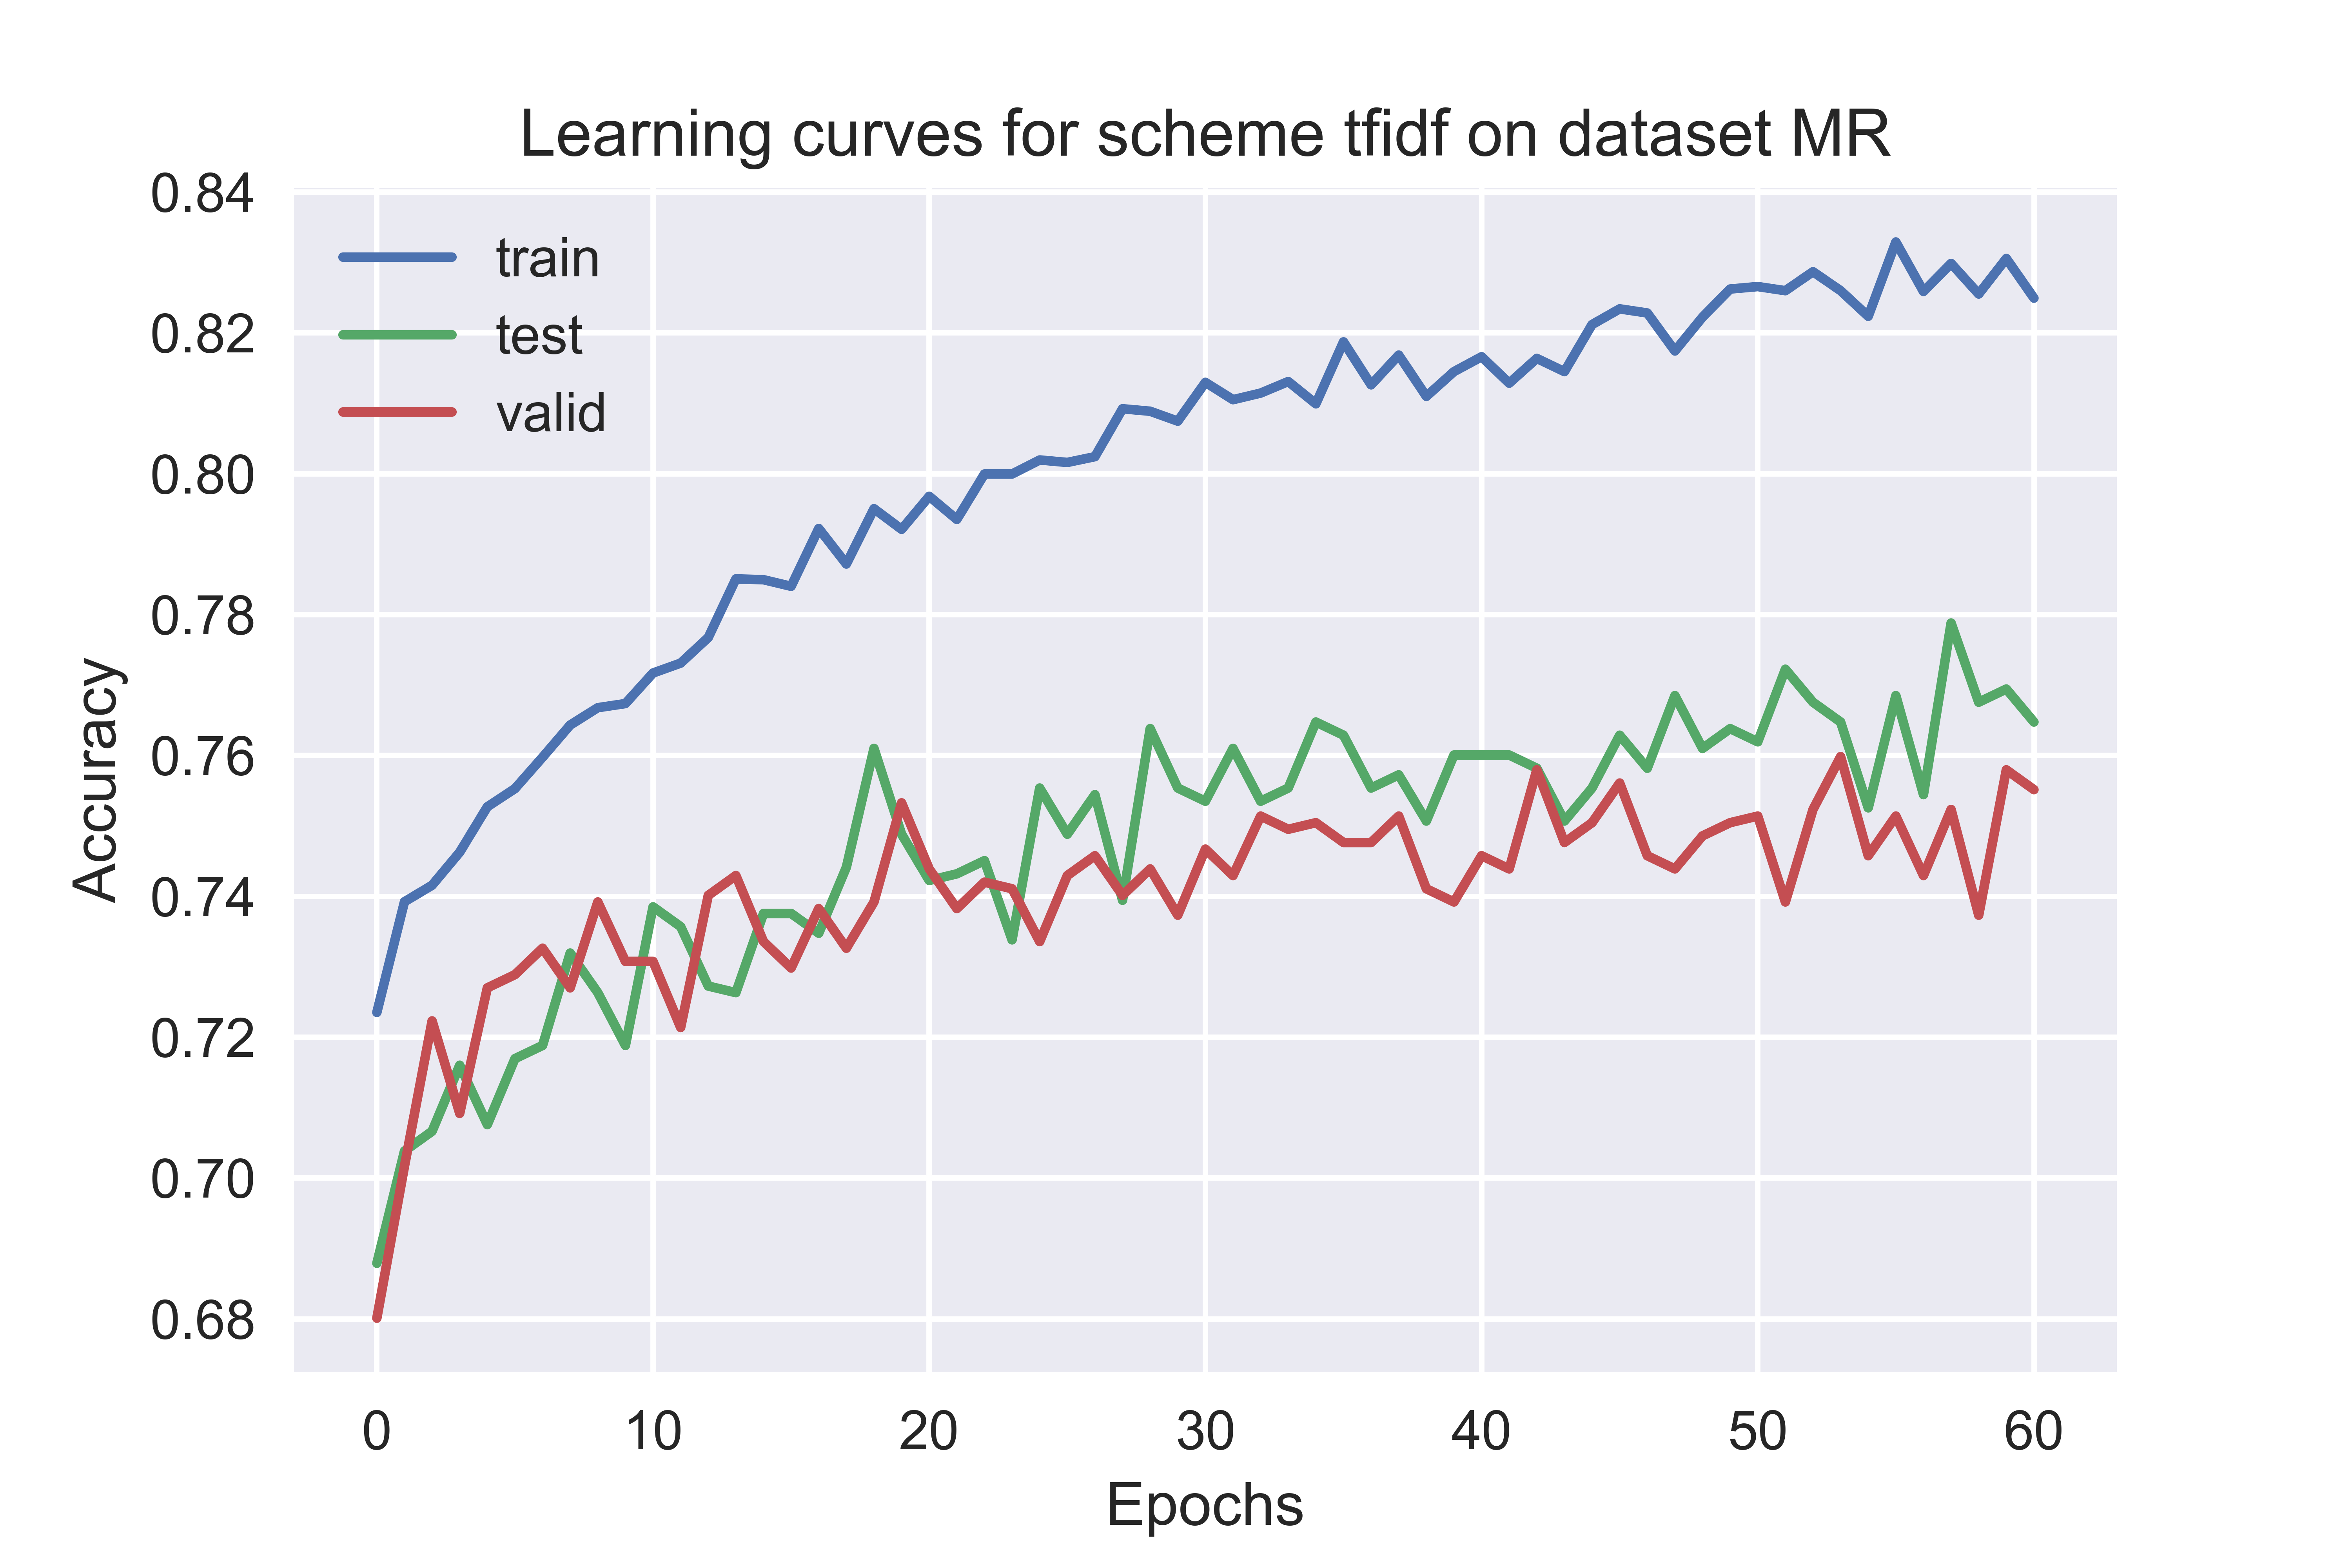
\includegraphics[width=0.8\textwidth]{images/learning_curve_MR_tfidf}}
    \caption[Learning curve for eLSA with tfidf weights on MR dataset]{Learning curve for eLSA with tfidf weights on MR dataset}
    \label{img:learning:curve}
    \end{figure}

    On figure \ref{img:learning:curve} we see a standard progress of accuracy through epochs. 
    We observe, that these curves are not entirely smooth as in batch gradient descent in neural networks.
    This is because we are not performing the exact gradient descent.
    The SVD part of eLSA is not deterministic and can be influenced by the weight $w'$.
    
    Recall from section \ref{sec:elsa:stopping} that we monitor the validation accuracy and stop the learning process when it plateaus. 

    \subsubsection{Multiple gradient steps}
    
    We perform an experiment, where we do multiple gradient steps on $w'$ for each loop. 
    This optimization routine is illustrated by algorithm \ref{algo:batch:multiw}.
    
    \begin{algorithm}[H]
        \KwData{$M$}
        \KwResult{trained $W$, $S$, $C$ }
        $w'^0 = 1$, $t=1$\;
        \While{performance is improving on validation dataset, $t$++}{
            recompute $S^t$ from $M \circ w'^{t-1}$\;
            compute embeddings $v^t$ from $M \circ w'^{t-1}$ with $S^t$\;
            fully train $C^t$ on $v^t$ and labels $y$\;
            \For{$0\leq i < m$}{
                update $W^t$: $w'^t = w'^{t-1} - \beta \frac{\partial E(C(S(M w'^{t-1}))}{\partial w'^{t-1}}$
            }
        }
        \caption{stochastic training of $w'$} \label{algo:batch:multiw}
    \end{algorithm}
    
    However this introduces another hyperparameter: number of performed $w'$ steps.
    We would like to to avoid new hyperparameters, so we do not spend too much resources on this experiment.
    Second problem with this approach is, that if we perform $m$ steps, the algorithm may be $m$ times slower. 
    This is a serious issue for $m>5$. 
    We perform experiments only for weighting scheme \texttt{None} with $200$ dimensional embedding and learning rate $0.1$.
    We perform $m=2$ and $m=5$ gradient steps and we present results in tables \ref{tab:multiw:notrec:2},
    \ref{tab:multiw:trec:2},\ref{tab:multiw:notrec:5} and \ref{tab:multiw:trec:5}.
    
    


\begin{table}[H]
\begin{center}

\begin{tabular}{lrrrr}
\toprule
{} &  CR &  MPQA &  MR &  SUBJ \\
\midrule
test  &  -0.01 &   0.00 &   \textbf{0.01} &   \textbf{0.01} \\
train &   0.02 &   0.00 &   0.01 &    -0.00 \\
valid &  -0.02 &   0.01 &  -0.01 &   0.00 \\
\bottomrule
\end{tabular}

\caption[Accuracy increase for 2 steps compared to 1 step]{Accuracy increase for 2 steps compared to 1 step}
\label{tab:multiw:notrec:2}
\end{center}
\end{table}




\begin{table}[H]
\begin{center}

\begin{tabular}{lrrrrrr}
\toprule
{} &  ABBR &  DESC &  ENTY &  HUM &  LOC &  NUM \\
\midrule
test  &     0.0 &     -0.01 &     -0.01 &     0.00 &    -0.01 &     \textbf{0.01} \\
train &     0.0 &      0.00 &      0.01 &     0.00 &     0.00 &     0.00 \\
valid &      -0.0 &     0.02 &     -0.00 &     0.01 &     0.00 &    -0.01 \\
\bottomrule
\end{tabular}

\caption[Accuracy increase for 2 steps compared to 1 step on TREC dataset]{Accuracy increase for 2 steps compared to 1 step on TREC dataset}
\label{tab:multiw:trec:2}
\end{center}
\end{table}




\begin{table}[H]
\begin{center}

\begin{tabular}{lrrrr}
\toprule
{} &  CR &  MPQA &  MR &  SUBJ \\
\midrule
test  &  -0.01 &   \textbf{0.01} &   \textbf{0.02} &   \textbf{0.01} \\
train &   0.03 &   0.01 &   0.01 &   0.01 \\
valid &  -0.02 &   0.01 &   0.00 &    -0.01 \\
\bottomrule
\end{tabular}

\caption[Accuracy increase for 5 steps compared to 1 step]{Accuracy increase for 5 steps compared to 1 step}
\label{tab:multiw:notrec:5}
\end{center}
\end{table}




\begin{table}[H]
\begin{center}

\begin{tabular}{lrrrrrr}
\toprule
{} &  ABBR &  DESC &  ENTY &  HUM &  LOC &  NUM \\
\midrule
test  &     0.0 &     -0.01 &     -0.00 &    -0.00 &     0.00 &     \textbf{0.01} \\
train &     0.0 &      0.01 &      0.01 &     0.00 &     0.01 &     0.01 \\
valid &     0.0 &      0.00 &      0.02 &    -0.01 &    -0.00 &     0.01 \\
\bottomrule
\end{tabular}

\caption[Accuracy increase for 5 steps compared to 1 step on TREC dataset]{Accuracy increase for 5 steps compared to 1 step on TREC dataset}
\label{tab:multiw:trec:5}
\end{center}
\end{table}



    We conclude, that making multiple gradient steps on $w'$ does not significantly nor consistently improve the accuracy and only makes the training process slower.
    The intuition, that multiple gradient steps on $w'$ may decrease the convergence time also showed to be wrong.


\begin{table}[H]
\begin{center}

\begin{tabular}{lrrrr}
\toprule
{} & CR & MPQA & MR & SUBJ \\
\$m\$ &      &       &      &       \\
\midrule
1  &     33 &      52 &     57 &      37 \\
2  &     32 &      43 &     45 &      46 \\
3  &     32 &      56 &     48 &      36 \\
4  &     33 &      68 &     63 &      39 \\
5  &     35 &      53 &     48 &      41 \\
\bottomrule
\end{tabular}

\caption[Number of needed training steps for different $w'$]{Number of needed training steps for different $w'$}
\label{tab:multyw:steps}
\end{center}
\end{table}


\begin{table}[H]
\begin{center}

\begin{tabular}{lrrrrrr}
\toprule
{} & ABBR & DESC & ENTY & HUM & LOC & NUM \\
\$m\$ &          &          &          &         &         &         \\
\midrule
1  &        32 &        38 &        38 &        72 &        38 &        48 \\
2  &        32 &        39 &        40 &        45 &        38 &        36 \\
3  &        32 &        48 &        35 &        38 &        32 &        38 \\
4  &        32 &        34 &        45 &        40 &        33 &        47 \\
5  &        32 &        37 &        36 &        32 &        37 &        52 \\
\bottomrule
\end{tabular}

\caption[Number of needed training steps for different $w'$ on TREC dataset]{Number of needed training steps for different $w'$ on TREC dataset}
\label{tab:multyw:steps:trec}
\end{center}
\end{table}

    The only relevant decrease in the number of required learning steps in tables \ref{tab:multyw:steps} and \ref{tab:multyw:steps:trec} can be seen for \texttt{TREC-HUM}.
    However this direction does not look very promising and we do not explore it further.
    